\documentclass[11pt,a4paper]{article}
\usepackage[T1]{fontenc}
\usepackage[utf8]{inputenc}
\usepackage[french]{babel}
\usepackage{lmodern,geometry,amsmath,booktabs,tabularx,xcolor,graphicx,fancyhdr,hyperref,listings}
\geometry{margin=2.15cm}
\definecolor{bleu}{HTML}{173B57}
\hypersetup{colorlinks=true,urlcolor=bleu,linkcolor=bleu}
\pagestyle{fancy}\fancyhf{}\fancyhead[L]{TP1 -- Étude de la consommation d'un core}\fancyhead[R]{M2 ESTel}\fancyfoot[C]{\thepage}
\setlength{\headheight}{15pt}
\setlength{\parindent}{0pt}\setlength{\parskip}{6pt}
\renewcommand{\arraystretch}{1.2}
\lstset{basicstyle=\ttfamily\footnotesize,breaklines=true,frame=single,columns=fullflexible}
\begin{document}
\hypersetup{pageanchor=false}\begin{titlepage}
{\large Université Côte d'Azur\\EUR DS4H -- Master 2 ESTel\\SMUEL302 -- Architecture multicores}
\vspace{2.1cm}

{\Huge\bfseries Étude de la consommation sur FPGA\par}
\vspace{0.5cm}
{\LARGE TP1 Opérateurs et traitement d'image\par}
\vspace{0.9cm}
{\Large Maxime Barbe\par}
\vspace{0.3cm}
2 novembre 2026

\vspace{1.2cm}
\begin{center}
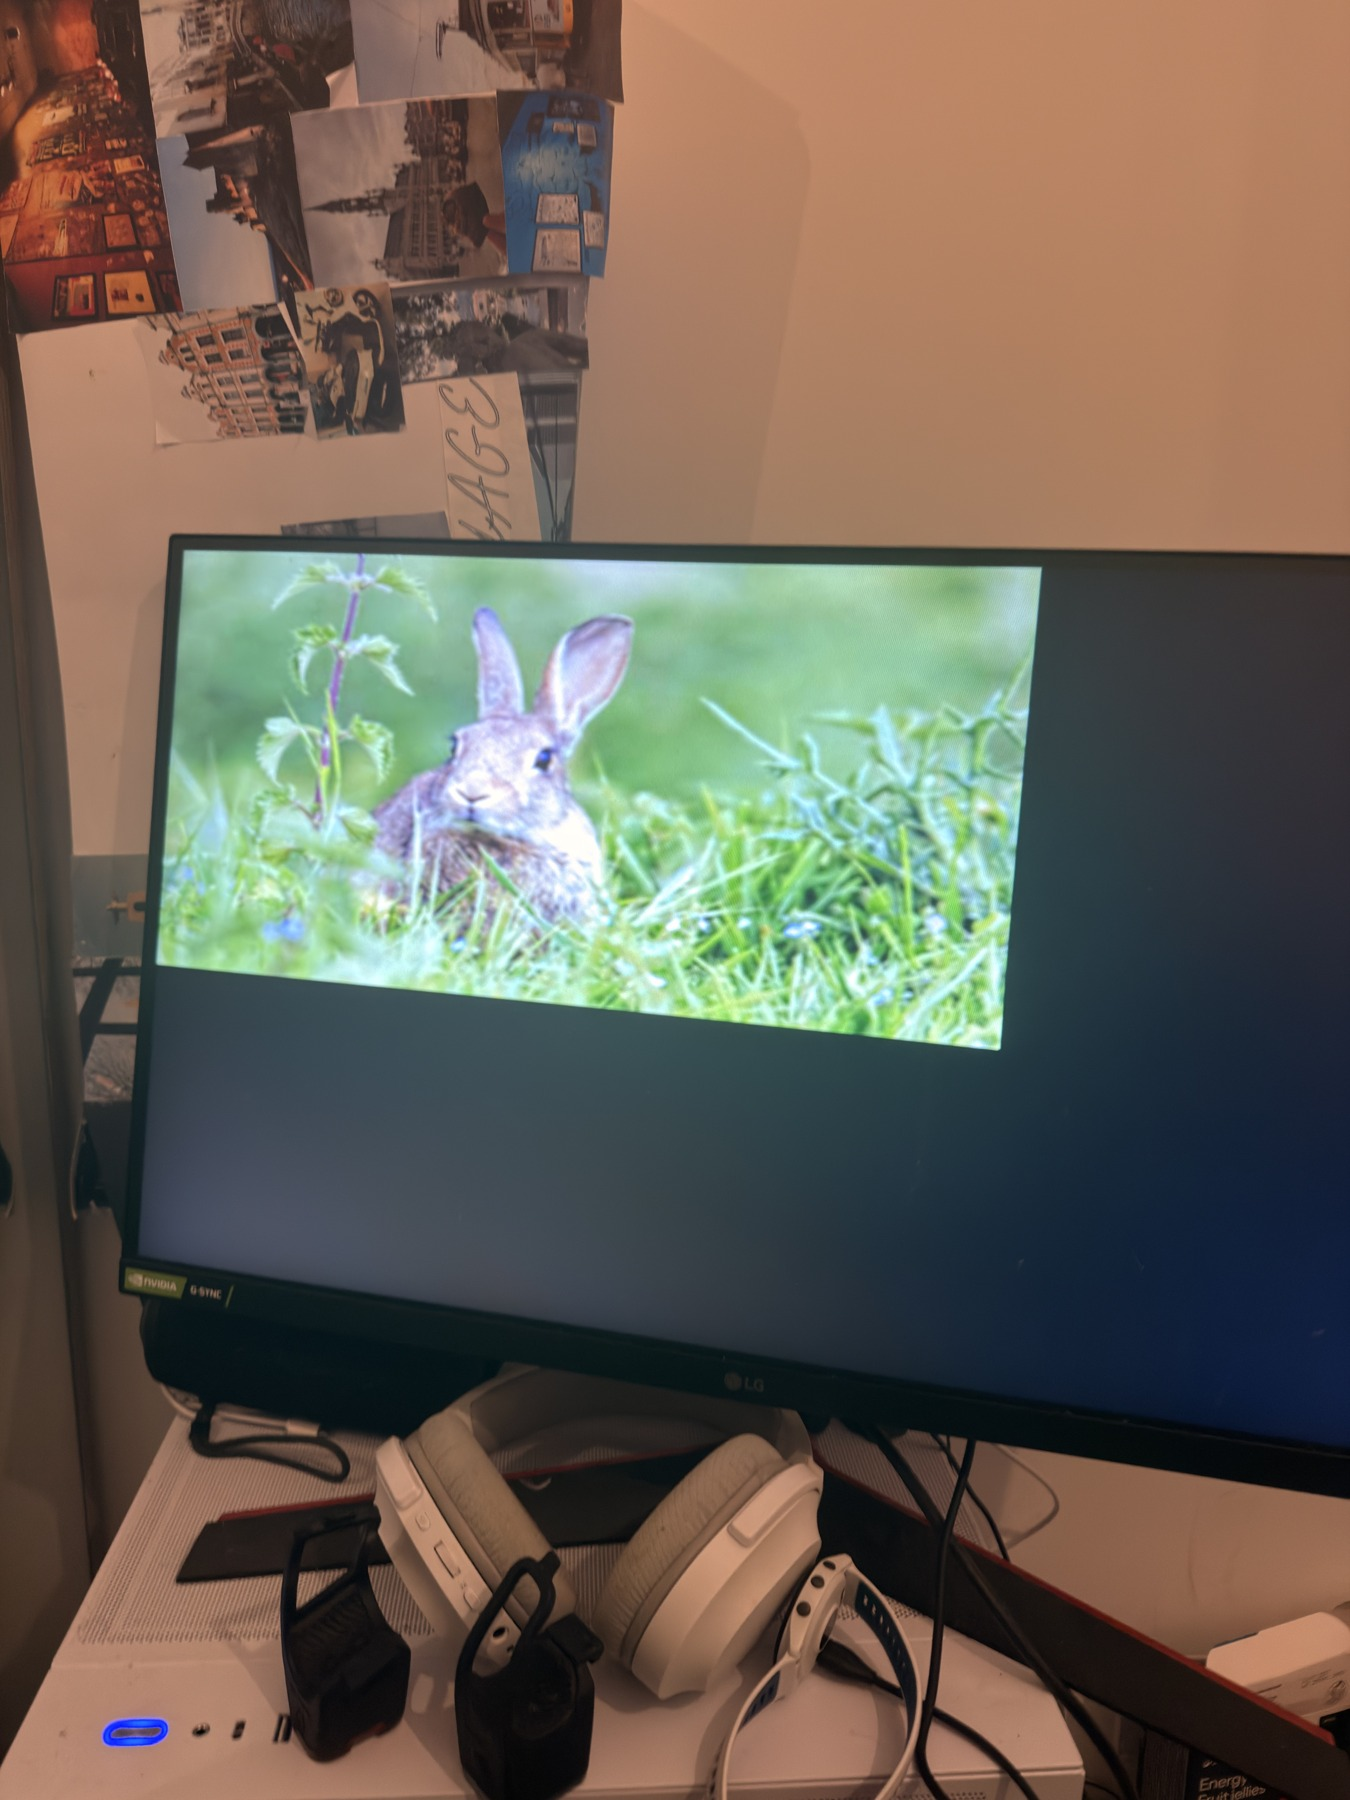
\includegraphics[width=0.70\linewidth,height=7cm,keepaspectratio]{images/affichage_on.jpg}
\end{center}
\vfill
\textbf{Plateforme :} Terasic DE10-Nano, Cyclone V 5CSEBA6U23I7.\\
\textbf{Outils :} Quartus Prime Lite 17.1, Power Analyzer, description VHDL/Verilog.

\end{titlepage}\hypersetup{pageanchor=true}

\section{Objectif et méthode}
Le TP étudie la relation entre architecture, débit et consommation. L'exercice 1 compare des opérateurs 32 bits, le pipeline et le parallélisme. L'exercice 2 applique ces principes à un filtre vidéo. L'exercice 3 réalise une chaîne complète sur FPGA et mesure son alimentation [1].

\subsection{Puissance, énergie et périmètre}
La puissance du circuit comprend une contribution statique et une contribution dynamique. La première subsiste sans commutations utiles ; la seconde dépend notamment de l'activité, de la capacité commutée, de la tension et de la fréquence. L'énergie se calcule sur une durée :
\[
 P=P_{\mathrm{stat}}+P_{\mathrm{dyn}},\qquad
 E=\int_0^T P(t)\,dt \simeq \overline P\,T.
\]
Pour $N$ opérations valides terminées pendant la fenêtre $T$ :
\[
 E_{\mathrm{op}}=\frac{\overline P T}{N}
 =\frac{\overline P}{R_{\mathrm{op}}}.
\]
Pour une chaîne vidéo continue de débit $r$ images/s, $E_{\mathrm{image}}\simeq\overline P/r$. Cette normalisation est indispensable : une architecture plus puissante peut néanmoins consommer moins d'énergie par résultat si elle termine davantage de travail.

Le Power Analyzer estime une puissance du composant selon son modèle et l'activité fournie. Le testeur d'alimentation de l'exercice 3 inclut la carte et les pertes en aval de son point de mesure. Ces deux périmètres ne sont pas directement comparables.

\subsection{Conditions d'une comparaison équitable}
Il faut conserver le composant, les contraintes, les conditions électriques et thermiques, une distribution d'entrées comparable et une fenêtre d'activité documentée. Le nombre d'opérations réellement terminées doit être compté après remplissage du pipeline. Le support du TP rappelle l'importance des stimuli et de l'import d'un fichier d'activité VCD dans Power Analyzer [2, diapositives 5--11].

\newpage
\begingroup\small\section{Exercice 1 Opérateurs pipeline et parallélisme}
\subsection{Conditions d'analyse}
Les opérateurs sont implantés sur le Cyclone V 5CSEBA6U23I7 avec Quartus Prime Lite 17.1. La consommation est estimée avec Power Analyzer en mode \emph{Vectorless}. L'indice de confiance \emph{Low} reflète l'absence d'activité de simulation représentative. Les valeurs de puissance sont donc des estimations du composant et ne constituent pas des mesures sur carte. Les valeurs de cet exercice ont été obtenues à l'aide de commandes exécutées dans le terminal, l'extraction à partir des fichiers de formes d'onde n'ayant pas pu être réalisée. Aucune activité issue de ces fichiers n'est donc revendiquée pour les estimations présentées.

\subsection{Addition entière signée 32 bits}
L'IP \texttt{LPM\_ADD\_SUB} réalise une addition signée sur 32 bits. Trois configurations sont étudiées : pipeline 1, 2 et 4.
\begin{center}
\begin{tabular}{@{}rrrrrr@{}}
\toprule
Pipeline & $f$ (MHz) & $P_{tot}$ (mW) & $P_{dyn,core}$ & $P_{stat,core}$ & E/S$^*$\\
\midrule
1 & 100,00 & 441,43 & 1,15 & 412,36 & 27,92\\
2 & 337,27 & 490,76 & 5,52 & 412,77 & 72,47\\
4 & 210,70 & 476,23 & 3,91 & 412,65 & 59,67\\
\bottomrule
\end{tabular}
\end{center}
$^*$E/S en mW, calculées par différence $P_{tot}-P_{dyn,core}-P_{stat,core}$ ; la fréquence de 100 MHz est une fréquence d'étude : TimeQuest n'y donnait pas de Fmax exploitable. TimeQuest donne respectivement 337,27 et 210,70 MHz pour les pipelines 2 et 4.

\subsection{Énergie par opération : calcul sous hypothèse de débit}
Pour un résultat valide par cycle en régime établi, $E_{op}=P/f$. La fenêtre de 1000 opérations est une fenêtre de calcul théorique, et non une séquence dont l'activité aurait été mesurée. En excluant le remplissage du pipeline, $T=N/f$ donne respectivement 10,00, 2,965 et 4,746~$\mu$s pour les trois fréquences. Les énergies suivantes sont des estimations normalisées sous cette hypothèse de débit :
\begin{center}
\begin{tabular}{@{}rrrr@{}}
\toprule
Pipeline & $E_{tot}$ (nJ/op) & $E_{dyn,core}$ (pJ/op) & $L/f$ nominal (ns)\\
\midrule
1 & 4,414 & 11,50 & 10,00\\
2 & 1,455 & 16,37 & 5,93\\
4 & 2,260 & 18,56 & 18,98\\
\bottomrule
\end{tabular}
\end{center}
Les latences $L/f$ supposent que la profondeur demandée est effectivement réalisée. Parmi ces points estimés, le pipeline 2 minimise l'énergie totale normalisée. Le pipeline 4 n'atteint pas une fréquence supérieure au pipeline 2 : la profondeur seule ne garantit pas une progression de Fmax après placement-routage. Les fréquences différentes empêchent d'attribuer toute variation de puissance au seul pipeline.

\newpage
\subsection{Addition flottante 32 bits}
L'IP \texttt{ALTFP\_ADD\_SUB} utilise un exposant de 8 bits, une mantisse de 23 bits, un pipeline de 14 et l'arrondi \emph{To Nearest}. La fréquence maximale retenue est 183,82 MHz. Deux fréquences sont comparées :
\begin{center}
\begin{tabular}{@{}rrrrr@{}}
\toprule
$f$ (MHz) & $P_{tot}$ (mW) & $P_{dyn,core}$ (mW) & $E_{tot}$ (nJ/op) & $E_{dyn,core}$ (pJ/op)\\
\midrule
100,00 & 448,09 & 8,97 & 4,481 & 89,70\\
183,82 & 467,32 & 16,48 & 2,542 & 89,65\\
\bottomrule
\end{tabular}
\end{center}
À 183,82 MHz, la puissance statique du c\oe{}ur est 412,61 mW ; le poste E/S déduit vaut 38,23 mW. La fréquence est multipliée par 1,8382 et la puissance dynamique par environ 1,8372. Cette évolution est compatible avec $P_{dyn}\simeq\alpha CV^2f$ à activité et tension comparables. L'énergie dynamique normalisée reste presque constante, tandis que le coût statique par opération baisse si le débit augmente.

L'énergie dynamique flottante, environ 89,65 pJ/op, dépasse les 11,50 à 18,56 pJ/op des additions entières étudiées. Le traitement des exposants, l'alignement, la normalisation et l'arrondi ajoutent de la logique. Cette comparaison reste liée aux architectures et au modèle d'activité retenus.

\subsection{Multiplication signée 32$\times$32 vers 64 bits}
Les trois variantes \texttt{LPM\_MULT} utilisent trois DSP. Les ressources et puissances obtenues sont :
\begin{center}
\begin{tabular}{@{}rrrrrrrr@{}}
\toprule
Pipeline & ALM & Reg. & DSP & $P_{tot}$ & $P_{dyn,core}$ & $P_{stat,core}$ & E/S\\
\midrule
1 & 24 & 0 & 3 & 532,58 & 8,23 & 413,13 & 111,22\\
2 & 24 & 0 & 3 & 530,84 & 6,50 & 413,11 & 111,22\\
4 & 46 & 161 & 3 & 532,81 & 8,72 & 413,13 & 110,96\\
\bottomrule
\end{tabular}
\end{center}
Toutes les puissances sont en mW. Les trois postes retrouvent le total annoncé aux arrondis d'affichage près ; pour le pipeline 2, leur somme vaut 530,83 mW contre 530,84 mW annoncés, soit un écart de 0,01 mW. Le pipeline 4 ajoute des ressources, tandis que le pipeline 2 a la puissance dynamique estimée la plus faible. Les fréquences des variantes 2 et 4 ne sont pas indiquées dans cette analyse : on n'en déduit pas un classement énergétique par opération.

Le rapport du pipeline 1 indique 100 MHz. Le Fitter annonce zéro registre pour les variantes 1 et 2. Ce compteur doit être interprété en tenant compte des registres éventuellement intégrés aux blocs DSP : il ne suffit pas à conclure que la latence est nulle. La latence effective doit être vérifiée dans l'implantation ou en simulation.

\subsection{Portée des résultats obtenus}
Les valeurs numériques ci-dessus sont des estimations Vectorless : aucune activité provenant des fichiers de formes d'onde n'a été importée. Elles permettent de comparer les configurations documentées sous leurs hypothèses de débit, mais pas d'établir une mesure expérimentale du coût énergétique de chaque opération. La comparaison chiffrée à plusieurs voies et la multiplication sans DSP ne figurent pas parmi les essais retrouvés. Leur analyse ci-après est donc théorique.

\newpage
\subsection{Parallélisme et énergie par opération}
Le pipeline réduit la longueur du chemin combinatoire entre registres et permet éventuellement d'augmenter la fréquence. Le parallélisme consiste à utiliser plusieurs opérateurs qui travaillent simultanément. Avec $w$ voies indépendantes, une fréquence $f$ et un résultat utile par voie et par cycle, le débit en régime établi est :
\[
 R_w=w f,\qquad E_{op,w}=\frac{P_w}{w f}.
\]
Le nombre de voies multiplie donc le débit idéal, mais pas nécessairement la puissance dans les mêmes proportions. Un modèle simplifié distingue une puissance fixe de plateforme et une contribution par voie :
\[
 P_w=P_{fixe}+wP_{voie}+P_{partage}(w),\qquad
 E_{op,w}=\frac{P_{fixe}}{w f}+\frac{P_{voie}}{f}
            +\frac{P_{partage}(w)}{w f}.
\]
Le terme $P_{partage}$ regroupe notamment les surcoûts d'horloge, d'interconnexion et d'interface. Le terme fixe par opération diminue quand $w$ augmente, à condition d'alimenter réellement toutes les voies. En revanche, les entrées/sorties, le routage ou une baisse de fréquence maximale peuvent limiter ce bénéfice.

\begin{center}
\begin{tabular}{@{}rrrr@{}}
\toprule
Voies & Débit idéal à 100 MHz & Énergie par opération & Nature\\
\midrule
1 & 100 Mop/s & $P_1/10^8$ & Relation de calcul\\
2 & 200 Mop/s & $P_2/(2\times10^8)$ & Relation de calcul\\
4 & 400 Mop/s & $P_4/(4\times10^8)$ & Relation de calcul\\
\bottomrule
\end{tabular}
\end{center}
Les puissances $P_2$ et $P_4$ ne sont pas remplacées par des nombres : elles doivent correspondre à leurs propres compilations et activités. Une simple multiplication de la puissance du circuit à une voie ferait notamment compter plusieurs fois sa part fixe.

À fréquence identique, deux voies améliorent l'énergie par résultat si $P_2<2P_1$ ; quatre voies l'améliorent si $P_4<4P_1$. Pour une comparaison à fréquences différentes, le critère devient $P_w/(w f_w)<P_1/f_1$. Ces conditions répondent à l'évolution attendue, sans attribuer un gain mesuré à une configuration non caractérisée.

\subsection{Comparaison entre blocs DSP et éléments logiques}
Les trois multiplieurs chiffrés utilisent chacun trois DSP. Ils illustrent une variation de pipeline, et non deux technologies d'implantation. Le paramètre \texttt{USE\_EAB=OFF} du schéma ne démontre pas que les DSP sont désactivés.

Une multiplication en DSP utilise les blocs arithmétiques dédiés ; une multiplication en éléments logiques construit le produit à partir des ressources logiques et du routage. Les critères à comparer sont la puissance totale, la puissance dynamique, les ALM, les DSP, la fréquence atteinte et l'énergie par résultat à débit comparable. Une préférence énergétique universelle ne peut pas être déduite de la seule nature du bloc : elle dépend du placement, de l'activité et de la fréquence.

La comparaison doit conserver deux entrées signées de 32 bits et une sortie de 64 bits. Pour la variante logique, le rapport Fitter doit confirmer l'absence de DSP. La latence effective doit être contrôlée, y compris les registres internes aux DSP, car le compteur de registres logiques n'en donne pas à lui seul une description complète.

\newpage
\subsection{Schéma Quartus des opérateurs entiers}
La figure~\ref{fig:schema-operateurs} montre le câblage des deux opérateurs à partir des mêmes entrées \texttt{A0} et \texttt{B0}, sur 32 bits, et d'une horloge commune \texttt{clk}. Les deux blocs utilisent une représentation signée et le paramètre \texttt{LPM\_PIPELINE} est réglé à 1.

\begin{figure}[htbp]
\centering
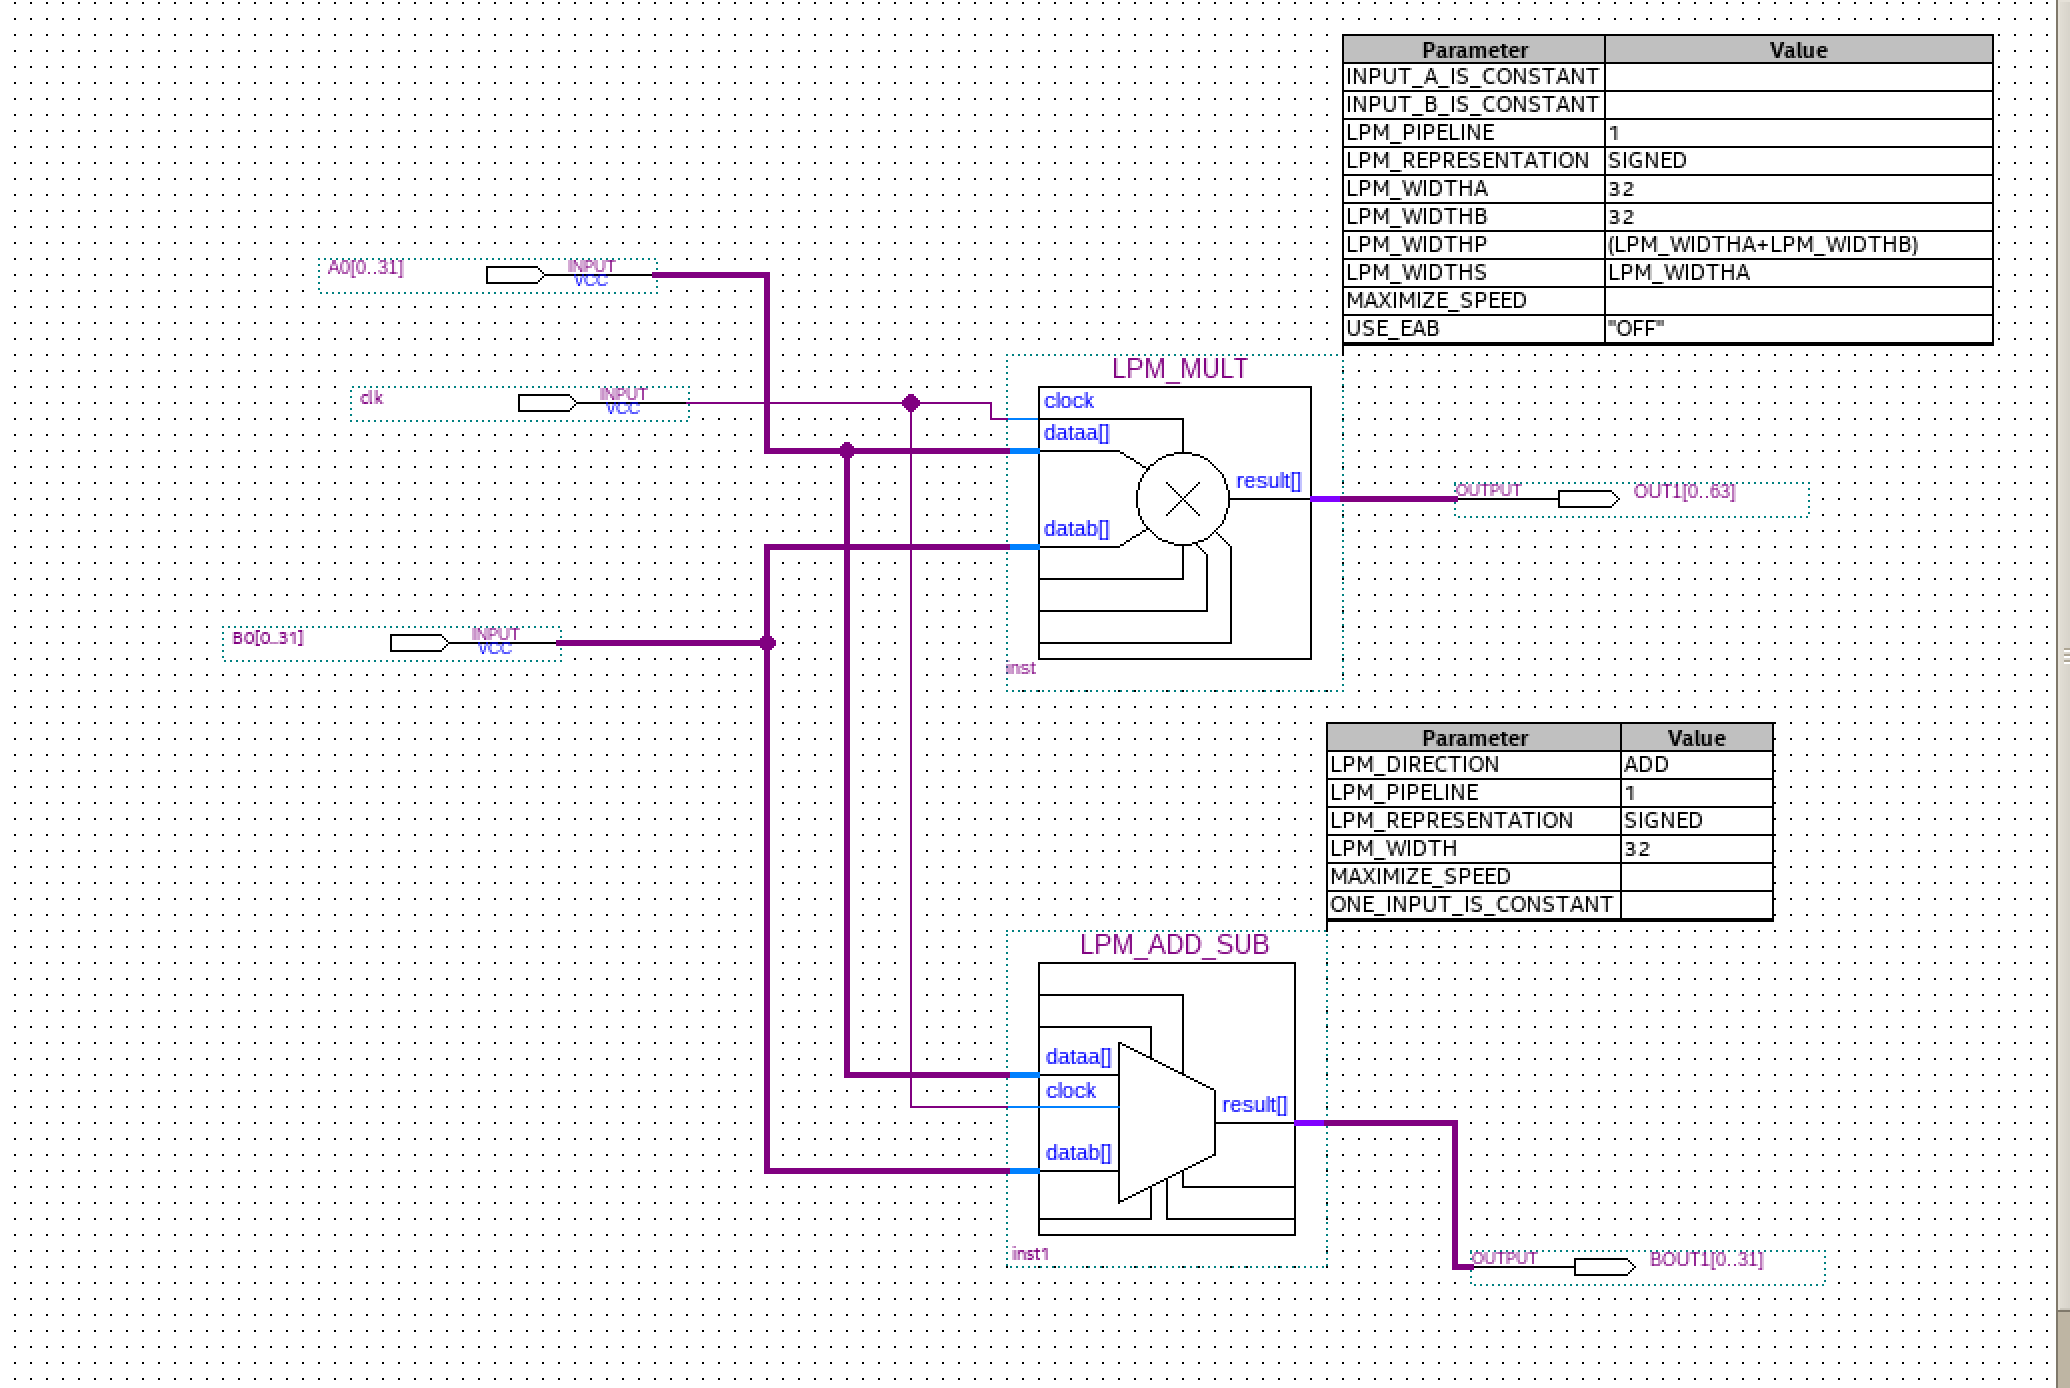
\includegraphics[width=\linewidth,height=14cm,keepaspectratio]{images/schema_operateurs_entiers.png}
\caption{Schéma Quartus d'un multiplieur signé 32$\times$32 vers 64 bits (\texttt{LPM\_MULT}) et d'un additionneur signé 32 bits (\texttt{LPM\_ADD\_SUB}, opération \texttt{ADD}), avec pipeline réglé à 1.}
\label{fig:schema-operateurs}
\end{figure}

Le produit est envoyé vers \texttt{OUT1[0..63]}, tandis que la somme est envoyée vers \texttt{BOUT1[0..31]}. La somme est conservée sur 32 bits ; un éventuel dépassement de capacité ne fournit pas de bit supplémentaire sur cette sortie.

Cette capture illustre le câblage ; elle ne documente pas à elle seule la configuration utilisée pour chaque ligne des tableaux de puissance. Les deux opérateurs sont présents simultanément dans ce schéma. Une estimation de puissance du projet complet inclurait leurs deux contributions et les ressources partagées. Pour comparer séparément addition et multiplication, les résultats de Power Analyzer doivent correspondre à chaque configuration isolée ou à un périmètre hiérarchique explicitement identifié. Le réglage de pipeline visible ne constitue pas, à lui seul, une vérification de la latence après synthèse.

\newpage
\endgroup\begingroup\small\section{Exercice 2 Architecture du filtre vidéo}
\subsection{Noyau et dimensionnement}
Le filtre proposé par l'énoncé [1] utilise le masque :
\[
 H=\frac1{10}
 \begin{bmatrix}
 1&1&1\\1&2&1\\1&1&1
 \end{bmatrix}.
\]
Pour chaque composante, la sortie est la somme pondérée des neuf pixels, divisée par 10. Les coefficients sont positifs et leur somme vaut 10 : le filtre réalise un lissage tout en préservant une région uniforme. Sur des entrées 8 bits :
\[
 0\leq S\leq 10\times255=2550.
\]
Une somme non signée de 12 bits suffit. Le fichier \texttt{filtre\_video.vhd} étend les entrées à 12 bits avant addition ; la multiplication centrale par 2 est un décalage. La division entière par 10 tronque la partie fractionnaire et la sortie reste dans $[0,255]$.

\subsection{IP isolée et chaîne complète}
La version \texttt{filtre\_video.vhd} du dépôt est combinatoire : neuf pixels 8 bits entrent en parallèle et une valeur filtrée en sort. Elle ne fournit ni voisinage mémoire ni synchronisation vidéo. Son temps de propagation doit être relevé après synthèse et placement-routage ; aucune valeur mesurée de ce délai n'a été retrouvée.

L'intégration de l'exercice 3 reconstruit le voisinage par deux buffers de ligne de 420 pixels et des registres horizontaux. Pour du RGB 24 bits, les buffers représentent logiquement :
\[
 2\times420\times24=20\,160\ \mathrm{bits}.
\]
Le flux utilise les pixels courants et précédents. Le centre du masque est donc situé en $(x-1,y-1)$ pour une sortie affichée en $(x,y)$. Les deux premières lignes et colonnes conservent le pixel initial. Ce choix évite de lire un pixel futur et doit être pris en compte pour comparer les images.

\begin{center}
\fbox{\begin{minipage}{0.92\linewidth}
\centering
ROM image RGB $\longrightarrow$ buffers de ligne et registres\\[3pt]
$\longrightarrow$ somme pondérée par canal $\longrightarrow$ division entière par 10\\[3pt]
$\longrightarrow$ sorties RGB et synchronisations HDMI alignées
\end{minipage}}
\end{center}

\subsection{Débit et énergie}
La chaîne intégrée traite jusqu'à un pixel par cycle de l'horloge vidéo dans la zone image. La lecture ROM prend un cycle ; le calcul et l'enregistrement des sorties en ajoutent un autre. Ce retard de chemin de données ne représente pas la latence complète depuis le premier pixel d'une image jusqu'au premier voisinage filtrable.

Le temps nécessaire pour disposer du premier voisinage comprend au moins deux lignes et deux colonnes. Dans la trame utilisée, les lignes comportent 800 périodes, y compris les zones de suppression vidéo ; la construction du voisinage s'étale donc sur le calendrier vidéo, pas seulement sur les 420 pixels utiles d'une ligne.

La puissance estimée ci-dessous concerne une autre version, à sortie enregistrée. La mesure de la section suivante concerne toute la plateforme. Une comparaison énergétique selon le débit exige encore une activité représentative et des contraintes temporelles complètes.

\newpage
\subsection{Synthèse et consommation du filtre à sortie enregistrée}
Le filtre est synthétisé dans le projet \texttt{TP1\_EXO2}. Le fichier \texttt{TP1\_EXO2.vhd} calcule la même somme pondérée, puis enregistre \texttt{somme/10} sur le front montant de \texttt{clk}. Il traite une composante 8 bits ; les neuf entrées totalisent 72 bits. Cette réalisation possède donc une sortie enregistrée, contrairement au fichier combinatoire du dépôt.

\begin{center}
\begin{tabular}{@{}lr@{}}
\toprule
Power Analyzer / Fitter & Valeur\\
\midrule
Puissance thermique totale estimée & \textbf{428,86 mW}\\
Puissance dynamique du c\oe{}ur & 1,24 mW\\
Puissance statique du c\oe{}ur & 412,26 mW\\
Puissance des E/S & 15,36 mW\\
ALM & 75\\
Registres & 8\\
Blocs DSP / bits mémoire & 0 / 0\\
Horloge déclarée & 100 MHz (période 10 ns)\\
\bottomrule
\end{tabular}
\end{center}
La somme des trois postes de puissance est bien $1{,}24+412{,}26+15{,}36=428{,}86$ mW. Le poste statique domine ce modèle du composant. Le total inclut les E/S : il ne représente pas uniquement la logique arithmétique du filtre, ni l'alimentation de toute la carte.

\textbf{Activité et confiance.} Le rapport classe l'estimation \emph{Low : user provided insufficient toggle rate data}. Aucun signal ne reçoit d'activité issue de simulation. Cette estimation doit être interprétée avec les limites du modèle d'activité Vectorless.

\textbf{Limite temporelle.} Le fichier \texttt{SDC1.sdc} impose une période de 10 ns. Cependant, TimeQuest indique 72 ports d'entrée et 8 ports de sortie non contraints ; les rubriques Fmax et setup ne contiennent aucun chemin analysé (\emph{No paths to report}). Les marges de largeur minimale d'impulsion ne donnent pas le délai critique du calcul. La période demandée ne permet donc pas d'affirmer que le filtre accepte réellement un résultat valide toutes les 10 ns.

Sous l'hypothèse d'un résultat par cycle validé, l'énergie se calcule avec $E_{\mathrm{résultat}}=P/f$ et $E_N=NP/f$. Ces expressions exigent un débit établi et une puissance correspondant à son activité ; les rapports retrouvés ne suffisent pas à établir ces deux conditions.

\newpage
\subsection{Débit demandé et coût par image du filtre isolé}
Pour une image de $N=M\times H$ pixels, un traitement monochrome à un résultat par cycle nécessite idéalement $N$ cycles utiles par image, après disponibilité des voisinages. En négligeant le remplissage et les interruptions :
\[
 T_{image}=\frac{N}{f},\qquad r_{max}=\frac{f}{N},\qquad
 E_{image}=P\frac{N}{f}.
\]
La latence d'un résultat et l'intervalle entre résultats sont deux grandeurs différentes : ajouter des étages peut augmenter la première tout en conservant un intervalle d'un cycle.

Pour l'image $420\times280$, on obtient $N=117\,600$. Les fréquences minimales de calcul utile suivantes sont des exigences de débit, pas des fréquences validées par TimeQuest :
\begin{center}
\begin{tabular}{@{}rrr@{}}
\toprule
Débit souhaité & Fréquence utile minimale $Nr$ & Durée d'une image $1/r$\\
\midrule
30 images/s & 3,528 MHz & 33,33 ms\\
60 images/s & 7,056 MHz & 16,67 ms\\
100 images/s & 11,760 MHz & 10,00 ms\\
\bottomrule
\end{tabular}
\end{center}
Ces chiffres décrivent une IP isolée recevant un pixel utile à chaque cycle. La chaîne HDMI possède un calendrier différent : pour une trame de $800\times525$, 60 images/s demanderaient 25,2 MHz, car les périodes hors image font aussi partie du balayage.

À titre de normalisation conditionnelle, si le filtre enregistré atteignait effectivement un résultat par cycle à 100 MHz et si sa puissance de 428,86 mW correspondait à cette activité, alors :
\[
 T_{image}=1{,}176\ \mathrm{ms},\qquad
 E_{image}=0{,}42886\times0{,}001176
 \simeq0{,}5043\ \mathrm{mJ}.
\]
Ce résultat n'est pas une énergie mesurée du filtre : la fréquence de fonctionnement n'est pas validée avec les contraintes d'interface et l'activité reste Vectorless. Il concerne une composante 8 bits, et non les trois canaux RGB ni l'ensemble de la plateforme.

\subsection{Évolution attendue avec le débit}
Dans un modèle où l'activité et la tension restent comparables, la puissance dynamique évolue approximativement avec la fréquence. Si le débit utile est proportionnel à $f$, une représentation simplifiée est :
\[
 P(r)\simeq P_{fixe}+k r,\qquad
 E_{image}(r)\simeq\frac{P_{fixe}}{r}+k.
\]
La part fixe par image diminue lorsque le débit augmente. Cette évolution suppose un fonctionnement continu avec toutes les images effectivement traitées ; elle ne prédit pas les gains d'un arrêt d'horloge ou d'une mise en veille entre images. Le seul point Power Analyzer disponible ne permet pas de mesurer une courbe $P(r)$ ni d'en identifier fiablement les coefficients.

\newpage
\subsection{Implémentation du filtre sous Quartus}
La figure~\ref{fig:quartus-filtre-source} présente les neuf entrées du filtre, le calcul de la somme pondérée et le registre de sortie commandé par \texttt{clk}.
\begin{figure}[htbp]
\centering
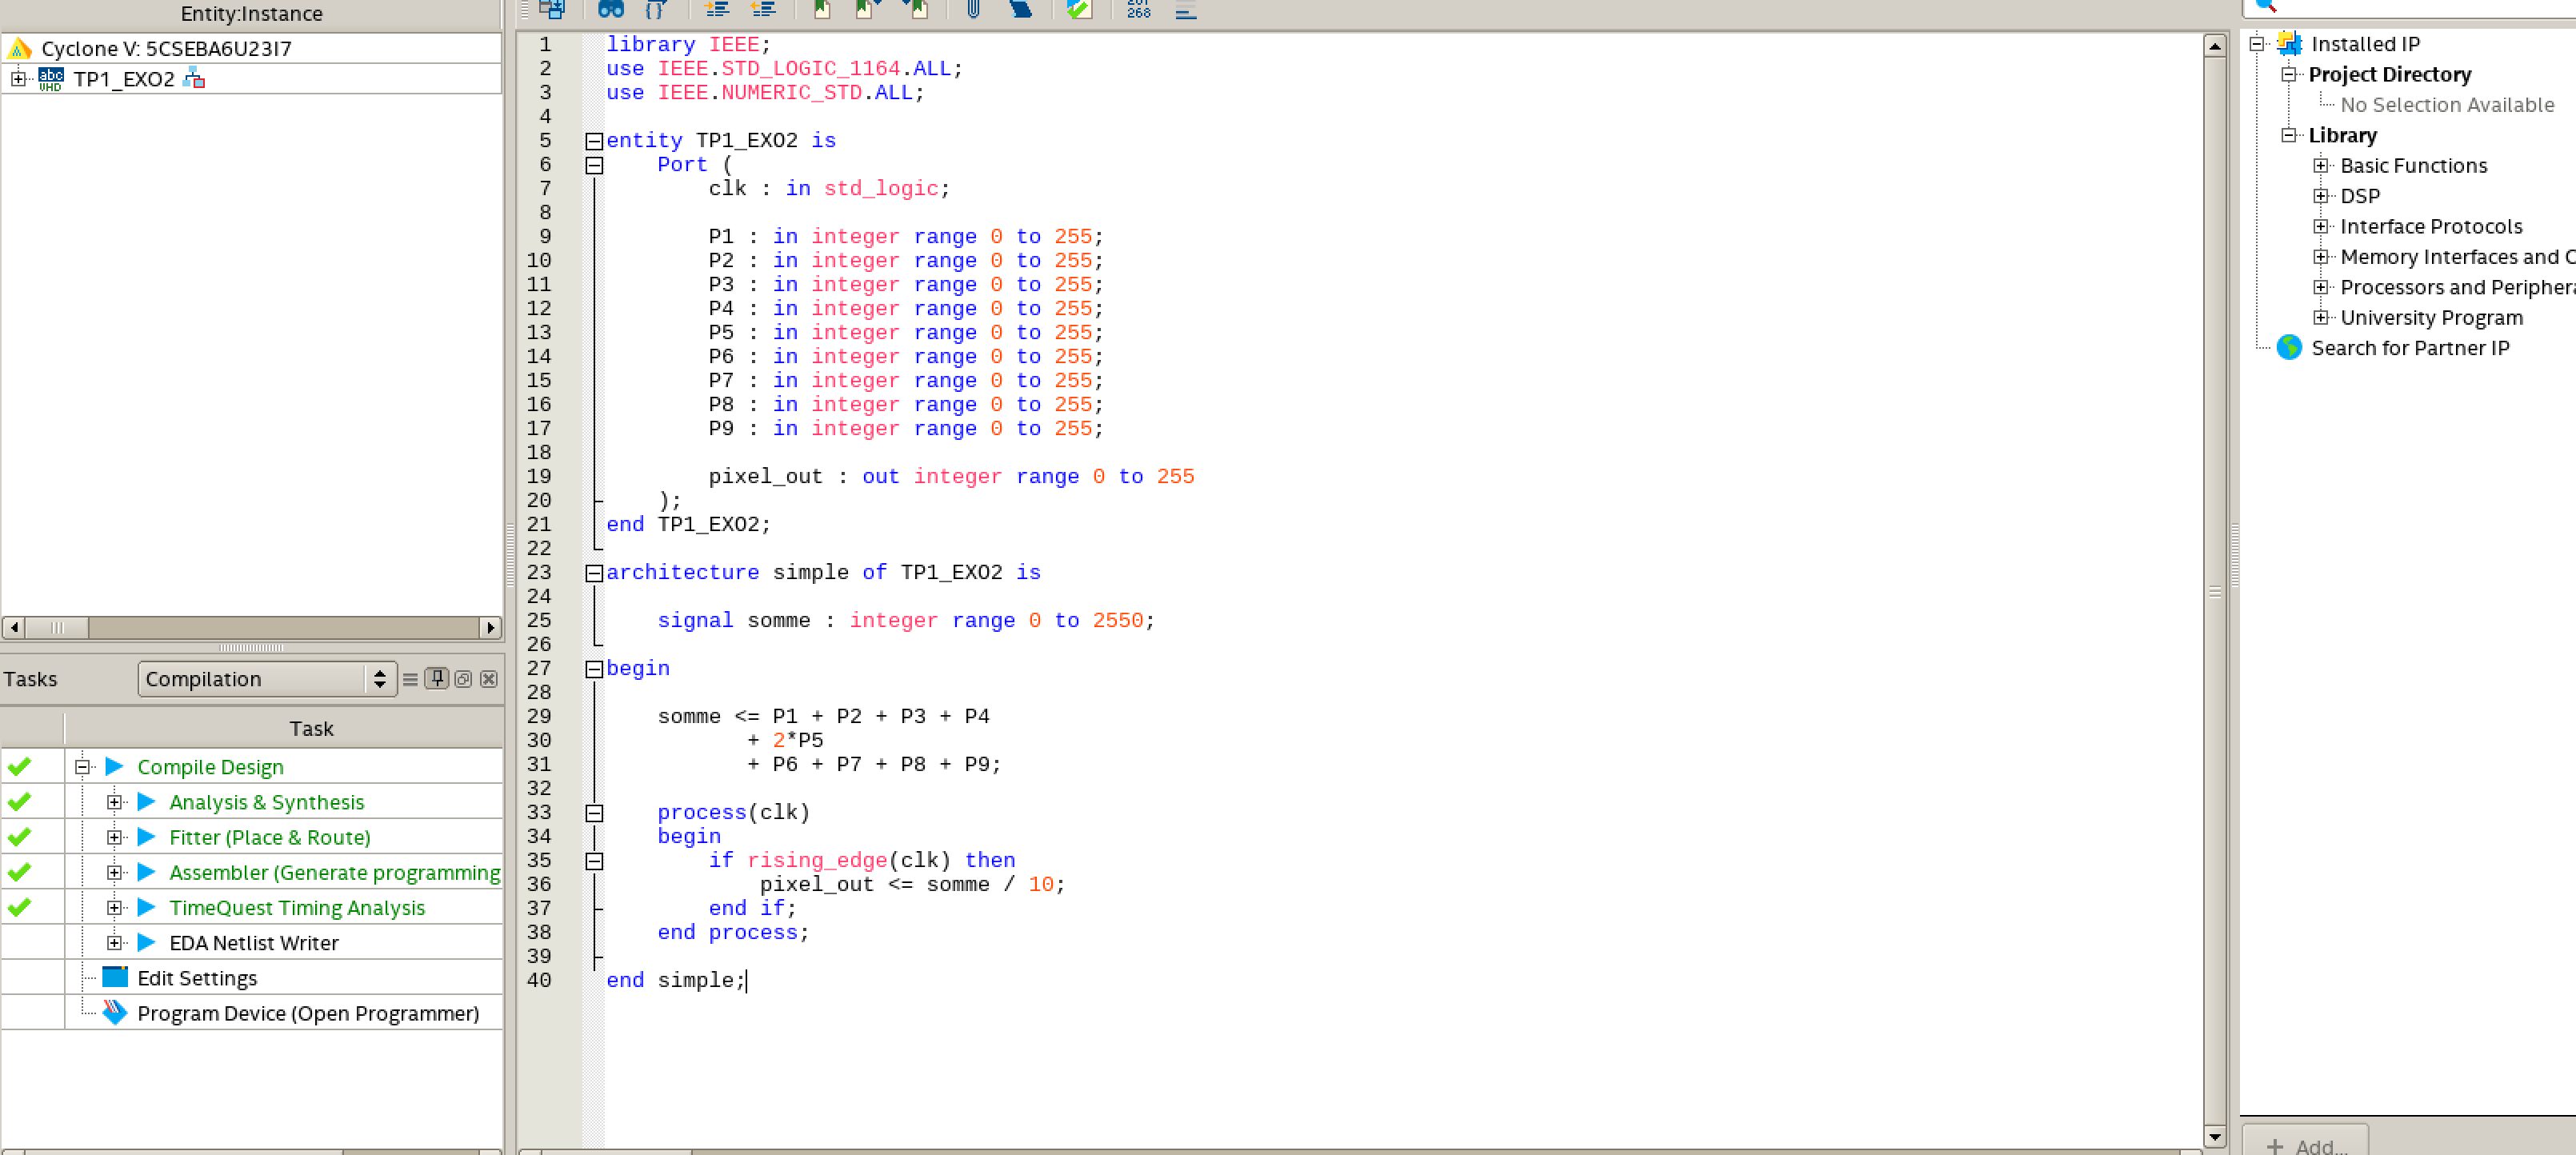
\includegraphics[width=\linewidth]{images/quartus_filtre_source.png}
\caption{Description VHDL du filtre à sortie enregistrée dans Quartus Prime Lite 17.1.}
\label{fig:quartus-filtre-source}
\end{figure}

La figure~\ref{fig:quartus-filtre-timequest} montre le panneau \emph{Datasheet Report -- Setup Times} de TimeQuest. Ces temps de setup aux ports ne constituent pas une mesure du délai critique complet du filtre ; leur interprétation dépend des contraintes d'interface.
\begin{figure}[htbp]
\centering
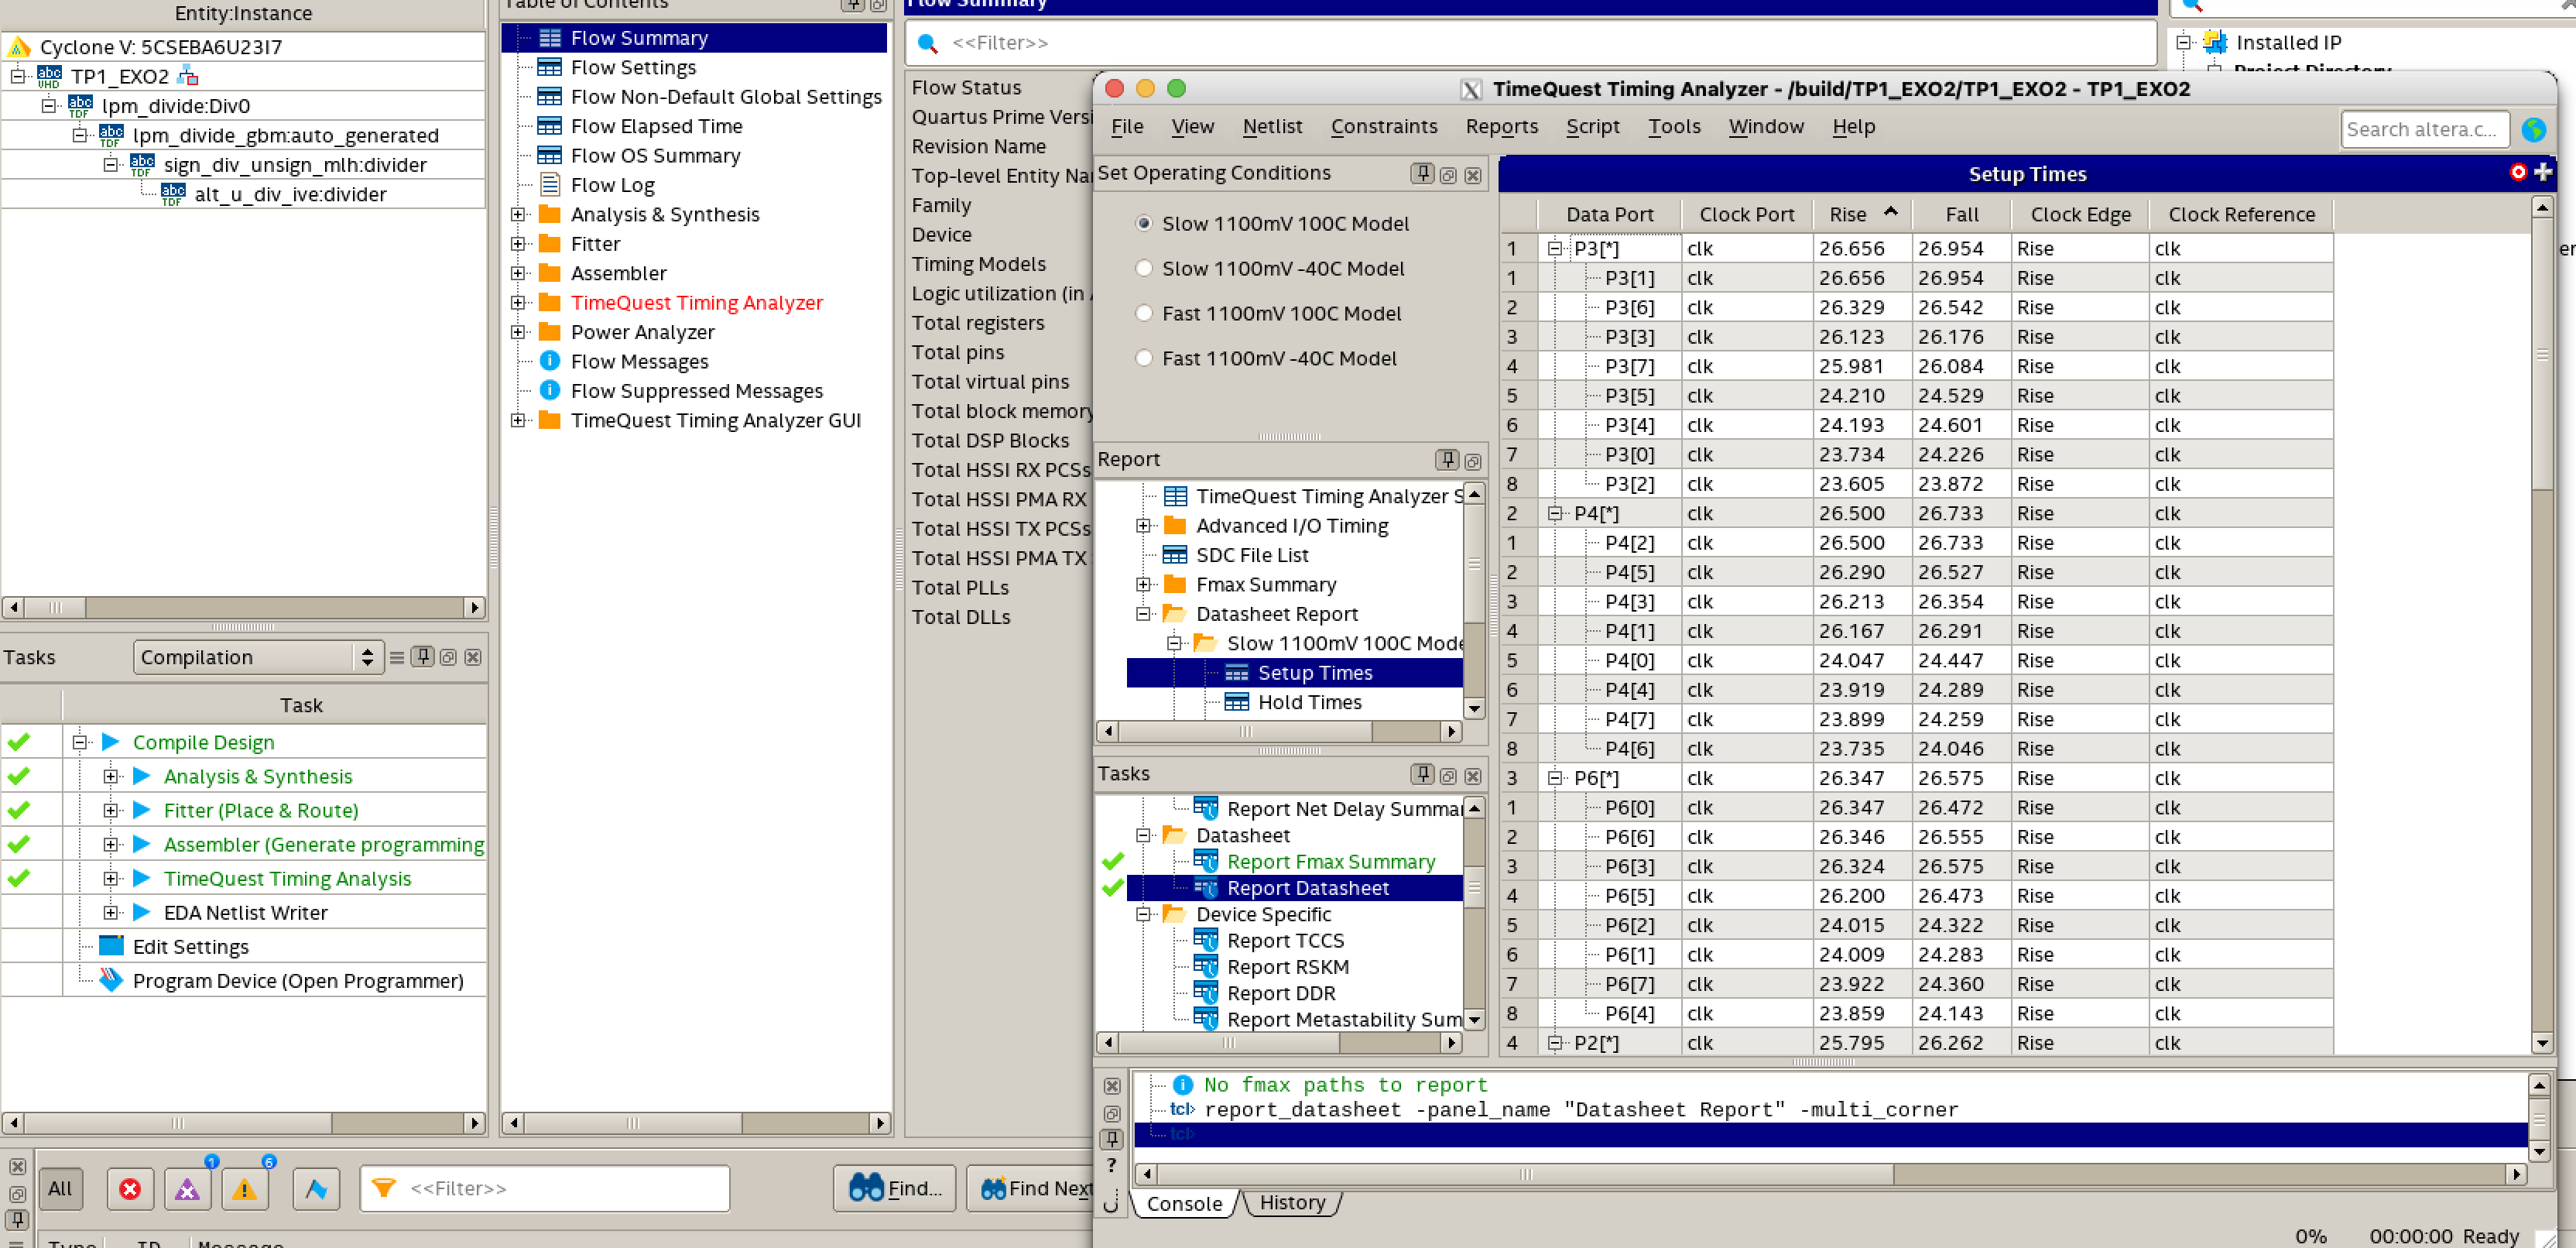
\includegraphics[width=\linewidth]{images/quartus_filtre_timequest.png}
\caption{Consultation des temps de setup aux ports du projet TP1\_EXO2 dans TimeQuest.}
\label{fig:quartus-filtre-timequest}
\end{figure}
\endgroup

\newpage
\section{Exercice 3 Réalisation sur DE10 Nano}
\subsection{Chaîne matérielle}
La réalisation s'appuie sur le FPGA Cyclone V 5CSEBA6U23I7 et le transmetteur HDMI ADV7513. L'image du lapin contient $420\times280=117\,600$ pixels RGB 24 bits stockés en ROM. Son adresse est $a=x+420y$ ; 17 bits permettent d'adresser la totalité de l'image.

\begin{center}
\begin{tabularx}{\linewidth}{@{}l X@{}}
\toprule
Fichier & Fonction\\
\midrule
\texttt{HDMI\_image\_student.vhd} & Entité supérieure, démarrage et raccordement des blocs.\\
\texttt{affichage\_image\_filtre.vhd} & Balayage, buffers, filtre et sorties vidéo.\\
\texttt{vga\_rom3.vhd} et \texttt{brom24b.mif} & Lecture de la ROM de l'image.\\
\texttt{I2C.vhd}, \texttt{i2c\_hdmi\_config.vhd} & Écriture des registres du transmetteur HDMI.\\
\texttt{affichage.qsf}, \texttt{affichage.sdc} & Configuration Quartus et contraintes.\\
\bottomrule
\end{tabularx}
\end{center}

\subsection{Calendrier vidéo}
L'horloge de 50 MHz est divisée par deux dans le code, donnant une horloge pixel nominale de 25 MHz. Les compteurs parcourent $800\times525$ positions pour une zone active $640\times480$. L'image occupe $420\times280$ positions ; le reste de la zone active est noir.
\[
 r=\frac{25\,000\,000}{800\times525}
   =59{,}5238\ \mathrm{images/s},\qquad
 T_{\mathrm{trame}}=16{,}8\ \mathrm{ms}.
\]
Ce débit vient du code et de l'horloge nominale. Il n'a pas été mesuré par un instrument. Les coordonnées et les synchronisations sont retardées pour accompagner les deux étages du chemin de données.

\subsection{Compilation et validation}
Le fichier de provenance du bitstream mentionne une compilation Quartus Lite 17.1 du 19 octobre 2026, sans erreur et avec huit avertissements :
\begin{center}
\begin{tabular}{@{}lr@{}}
\toprule
Ressource ou marge contrainte & Résultat\\
\midrule
ALM & 543 / 41\,910\\
Blocs RAM & 351 / 553\\
Bits mémoire & 2\,842\,560 / 5\,662\,720\\
Blocs DSP & 1 / 112\\
Marge setup minimale analysée & +5,925 ns\\
Marge hold minimale analysée & +0,113 ns\\
\bottomrule
\end{tabular}
\end{center}
Les délais externes de deux entrées et trente sorties ne sont pas entièrement contraints. Les marges internes positives ne constituent donc pas une validation temporelle complète des interfaces.

Les bancs vidéo, I2C et démarrage vérifient respectivement les pixels et les synchronisations, la configuration du transmetteur et la séquence de réinitialisation. Leur réussite est consignée dans le dépôt. Les photos attestent l'affichage, mais ne vérifient pas chaque pixel filtré.

\newpage
\subsection{Observation sur carte}
SW0 sur ON libère le reset : le lapin apparaît à l'écran. SW0 sur OFF maintient le circuit en réinitialisation : l'écran est noir. Ces états ont été confirmés lors du travail sur la carte, le 19 octobre.

\begin{center}
\begin{minipage}{0.47\linewidth}
\centering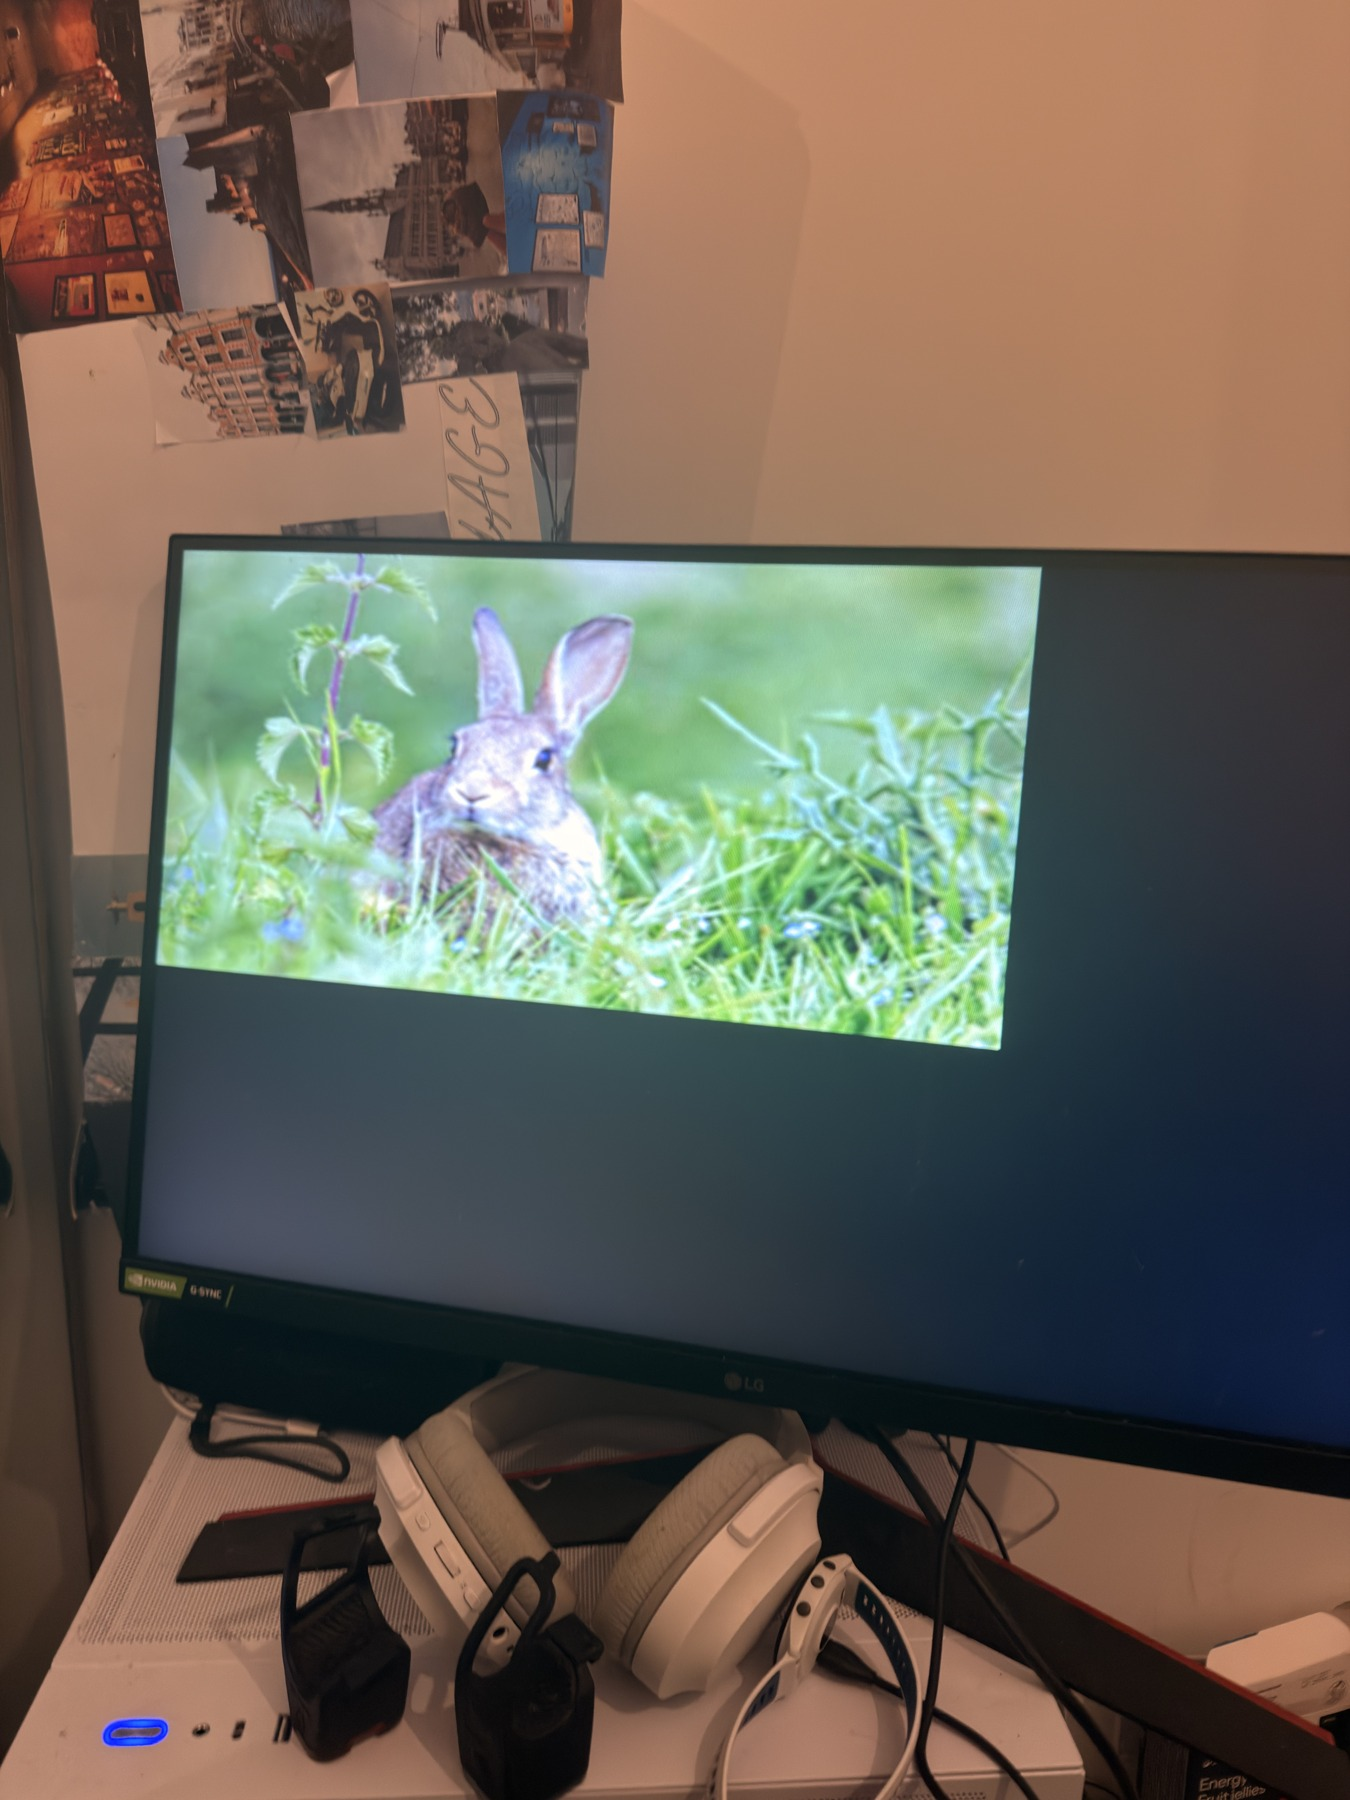
\includegraphics[width=\linewidth,height=7cm,keepaspectratio]{images/affichage_on.jpg}\\
\small SW0 ON : image affichée.
\end{minipage}\hfill
\begin{minipage}{0.47\linewidth}
\centering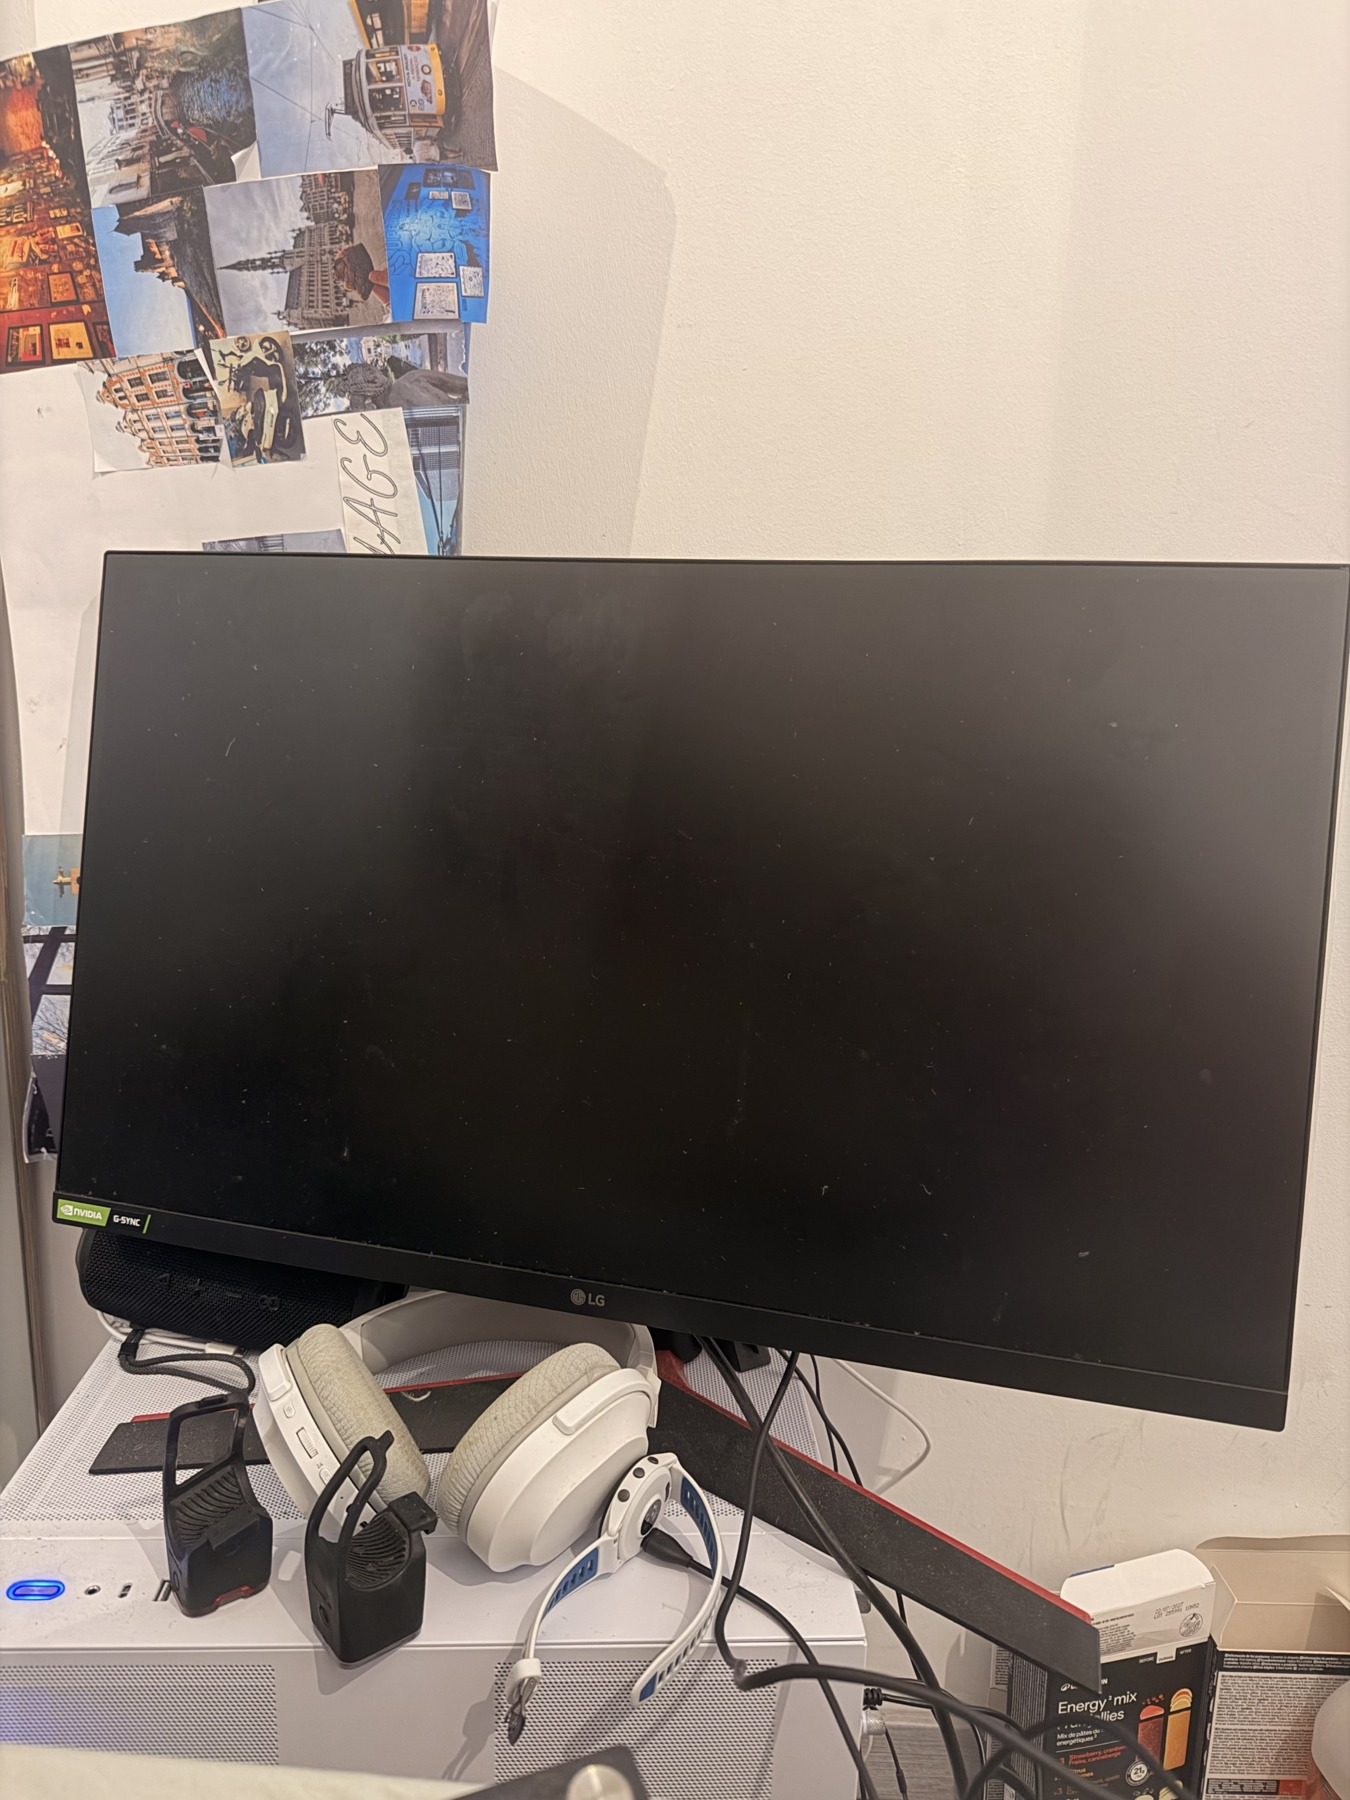
\includegraphics[width=\linewidth,height=7cm,keepaspectratio]{images/affichage_off.jpg}\\
\small SW0 OFF : écran noir.
\end{minipage}
\end{center}

\subsection{Montage et relevés de puissance}
Le montage déclaré est : \textbf{port USB du PC $\rightarrow$ testeur RUI DENG UM25C $\rightarrow$ entrée DC 5 V de la DE10-Nano}. Le testeur observe l'entrée d'alimentation de la plateforme, avec les pertes du câble situé en aval. Il n'isole pas le FPGA, le filtre ou le transmetteur HDMI.

\begin{center}
\begin{tabular}{@{}llrrr@{}}
\toprule
Photographie & Niveau observé & $U$ (V) & $I$ (A) & $UI$ (W)\\
\midrule
IMG\_0568 & Haut & 4,997 & 0,6293 & 3,144612\\
IMG\_0566 & Bas & 4,996 & 0,6240 & 3,117504\\
IMG\_0572 & Haut & 5,004 & 0,6301 & 3,153020\\
IMG\_0573 & Bas & 5,005 & 0,6238 & 3,122119\\
\bottomrule
\end{tabular}
\end{center}
Les puissances sont recalculées à partir des valeurs de tension et de courant lisibles sur les photos. La précision d'affichage du testeur ne constitue pas une incertitude métrologique ; les décimales des produits sont conservées pour rendre le calcul reproductible.

\subsection{Courant retenu et énergie par image}
Le courant retenu pour la plateforme est d'environ \textbf{0,6 A}, valeur validée par l'enseignante. Les relevés du tableau montrent les niveaux haut et bas de la consommation autour de ce niveau de fonctionnement. Ils ne constituent pas une mesure séparée de la consommation du filtre.

Avec une alimentation nominale de 5 V, la puissance correspondante est :
\[
 P_{\mathrm{nom}}\simeq U_{\mathrm{nom}}I_{\mathrm{retenu}}
 =5\times0{,}6=3\ \mathrm{W}.
\]
L'énergie par trame au débit nominal vaut donc :
\[
 \boxed{E_{\mathrm{image}}\simeq\frac{3}{59{,}5238}
 =0{,}0504\ \mathrm{J/image}\approx50\ \mathrm{mJ/image}.}
\]

\newpage
\section{Discussion et conclusion}
\subsection{Interprétation des niveaux haut et bas}
Le calcul nominal donne 50,4 mJ, mais le résultat est présenté comme environ 50 mJ par trame, car le courant de référence de 0,6 A est arrondi. Les photographies donnent des instantanés plus précis, entre 0,6238 et 0,6301 A, pour des puissances calculées entre 3,1175 et 3,1530 W. Leur moyenne arithmétique n'est pas une moyenne temporelle sur une campagne instrumentée.

L'observation principale est une consommation globale de l'ordre de 0,6 A, avec un niveau haut et un niveau bas visibles sur le testeur. Cette lecture est celle retenue après validation par l'enseignante. Les états ON et OFF de SW0 décrivent séparément l'affichage et la réinitialisation ; ils ne suffisent pas à attribuer une différence de puissance au seul traitement d'image.

Les quatre instantanés ne permettent ni d'isoler l'énergie du filtre ni d'établir une incertitude statistique robuste sur les fluctuations. La grandeur caractérisée reste l'alimentation de la plateforme, comprenant les pertes du câble en aval du testeur. Aucun gain énergétique propre au filtre n'est déduit de la différence entre les niveaux haut et bas.

\begin{center}
\begin{minipage}{0.47\linewidth}
\centering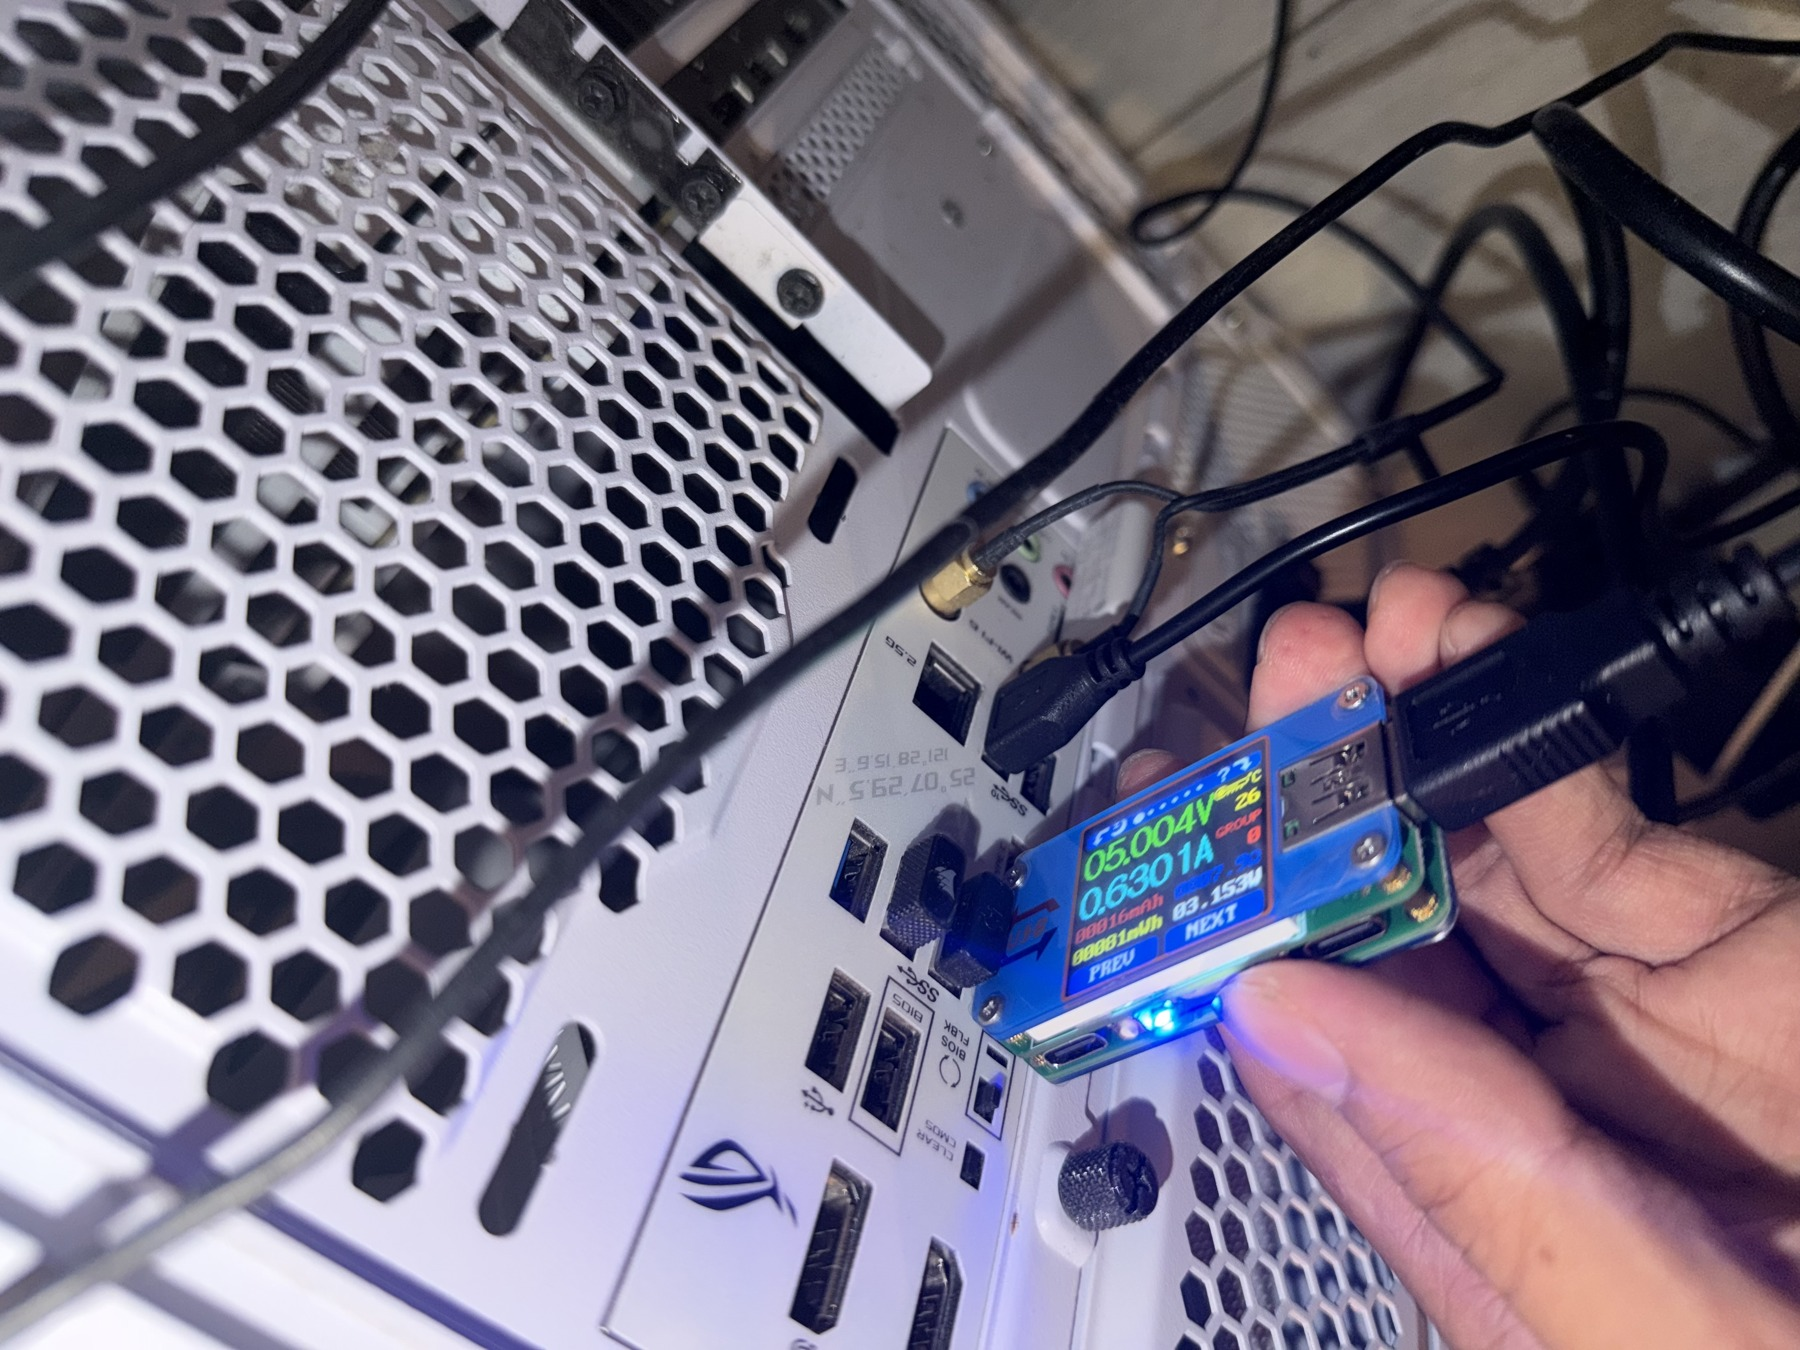
\includegraphics[width=\linewidth,height=5cm,keepaspectratio]{images/mesure_on.jpg}\\
\small IMG\_0572 : niveau haut, 5,004 V et 0,6301 A.
\end{minipage}\hfill
\begin{minipage}{0.47\linewidth}
\centering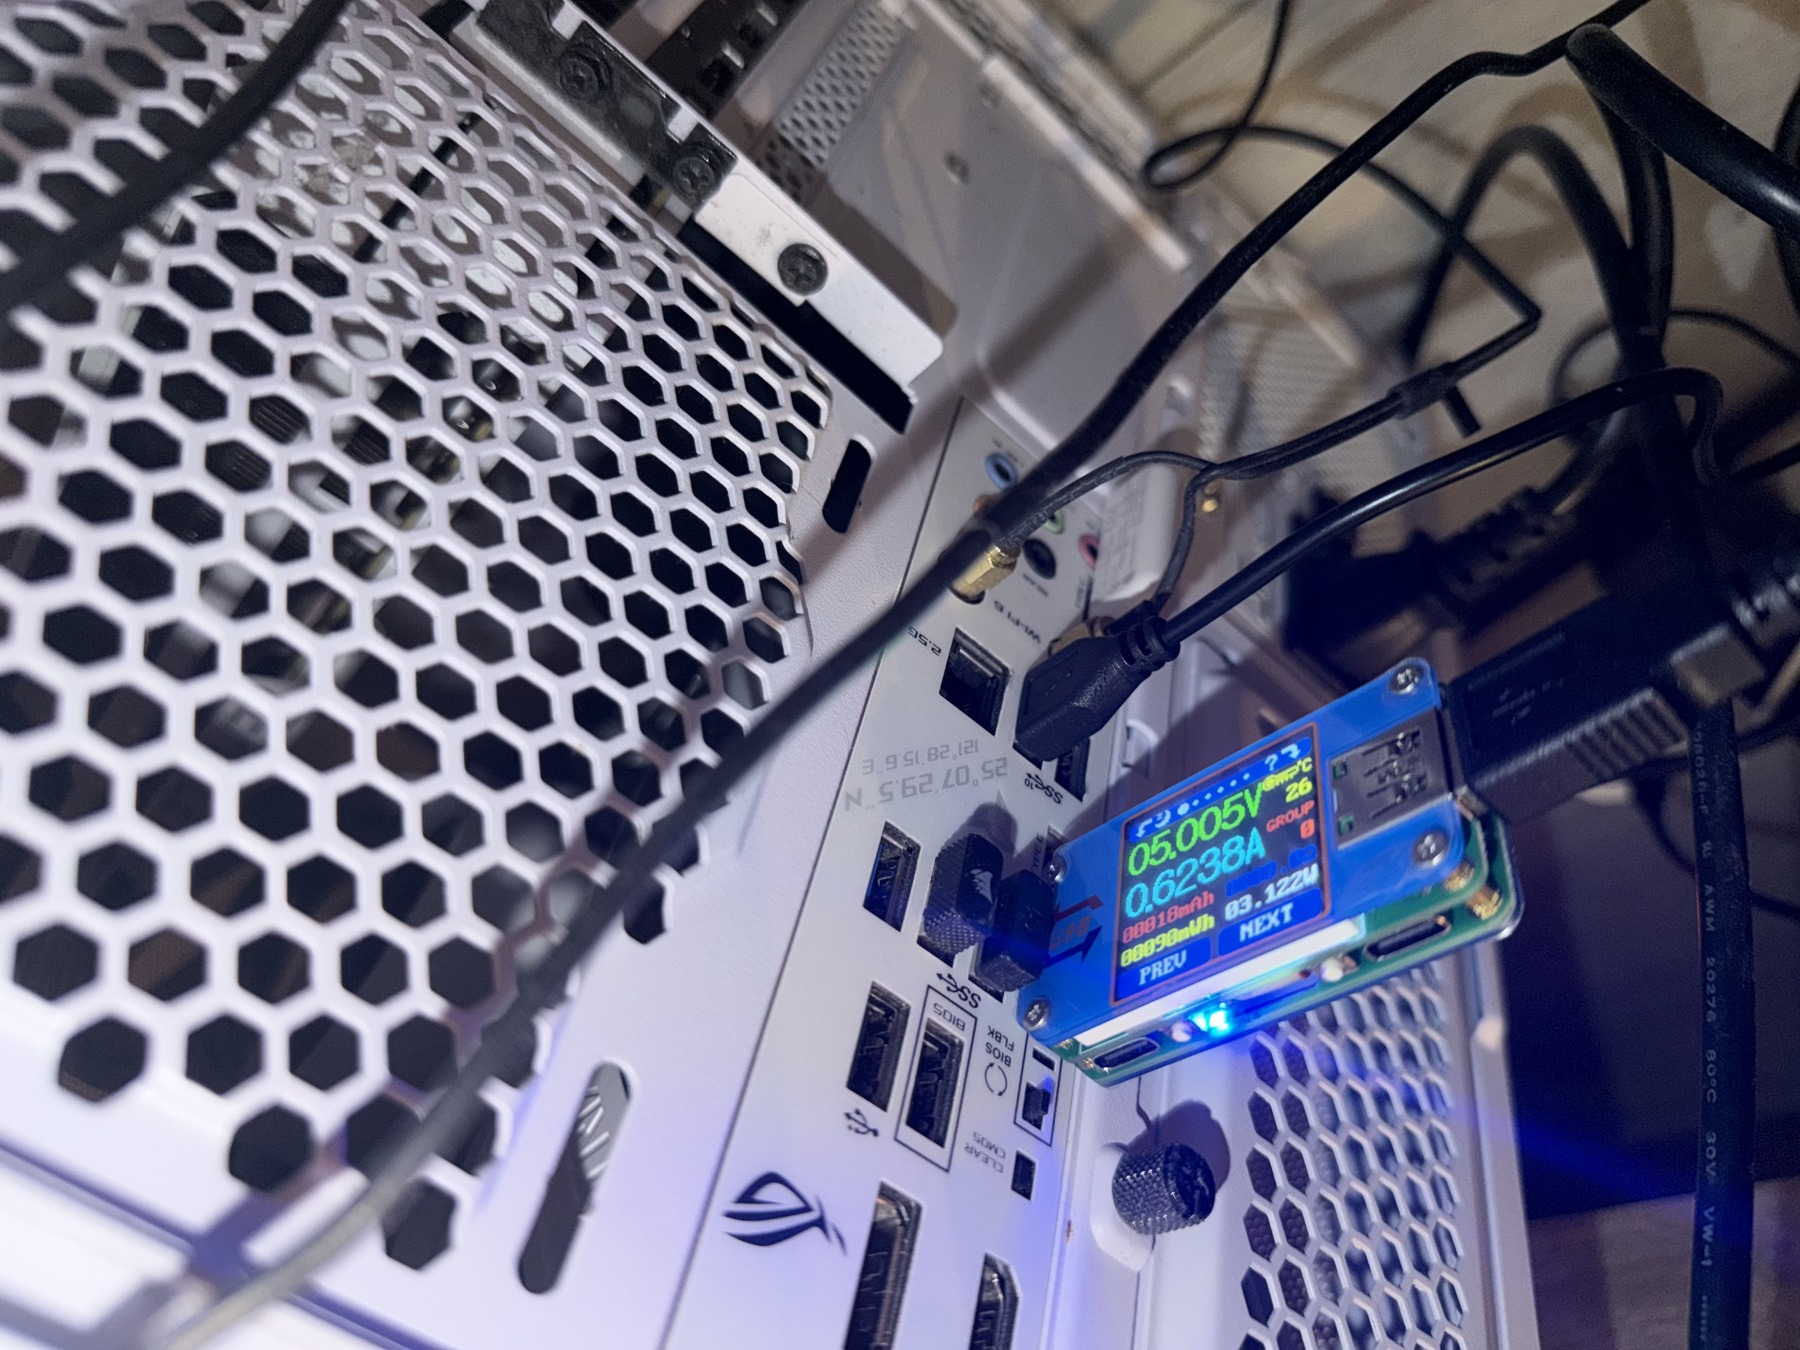
\includegraphics[width=\linewidth,height=5cm,keepaspectratio]{images/mesure_off.jpg}\\
\small IMG\_0573 : niveau bas, 5,005 V et 0,6238 A.
\end{minipage}
\end{center}

\subsection{Conclusion}
La chaîne réalisée stocke une image en ROM, construit un voisinage 3$\times$3, effectue un lissage RGB et génère une sortie HDMI. L'affichage sur carte est documenté. Le courant retenu et validé par l'enseignante est d'environ \textbf{0,6 A}. Sous 5 V, il correspond à une puissance nominale d'environ \textbf{3 W}, soit un ordre de grandeur de \textbf{50 mJ par trame} à 59,52 images/s. Les niveaux haut et bas observés décrivent les variations autour de ce courant ; ils ne mesurent pas isolément la consommation du filtre.

Ce résultat valide une première caractérisation de la plateforme. Le filtre enregistré dispose aussi d'une estimation Quartus de 428,86 mW, à faible confiance. L'étude des opérateurs montre l'intérêt du pipeline 2 pour l'énergie totale normalisée de l'addition entière. Les résultats restent conditionnés par le modèle d'activité, le débit effectivement validé et le périmètre de mesure.

Une intelligence artificielle a été utilisée comme aide à la rédaction et à la reformulation de ce rapport.

\newpage
\section{Bilan des réponses et reproduction des calculs}
\begin{center}
\begin{tabularx}{\linewidth}{@{}l X@{}}
\toprule
Question & Résultat et statut\\
\midrule
1.1 Addition entière et flottante & Puissances estimées documentées et énergies normalisées ; activité Vectorless et hypothèse d'un résultat par cycle.\\
1.2 Parallélisme & Modèle de débit et conditions de réduction de l'énergie ; aucune puissance à plusieurs voies mesurée.\\
1.3 DSP et éléments logiques & Trois variantes DSP chiffrées ; comparaison technologique explicitée, sans essai logique chiffré.\\
2 Filtre vidéo & Masque, architecture, ressources et puissance estimée ; calculs conditionnels du débit et de l'énergie, délai critique non validé.\\
3 Plateforme FPGA & Affichage et photographies, courant retenu d'environ 0,6 A, puissance nominale d'environ 3 W et énergie d'environ 50 mJ par trame.\\
\bottomrule
\end{tabularx}
\end{center}

\subsection{Méthode de calcul vérifiable}
Les tableaux CSV associés distinguent les valeurs reprises des rapports et les résultats calculés. Le script \texttt{scripts/calculs.py} reproduit les divisions $P/f$, les produits $UI$, les moyennes des niveaux observés et le calcul nominal de l'énergie par trame. Il ne lance pas de nouvelle estimation Power Analyzer et ne reconstitue aucune activité manquante.

Pour les estimations Quartus, l'utilisation du terminal sert à lancer les outils et à lire leurs rapports ; elle ne remplace pas le fichier d'activité de simulation. La commande suivante est un exemple de compilation du projet existant, à exécuter depuis son dossier :
\begin{lstlisting}
quartus_sh --flow compile affichage
\end{lstlisting}
Le projet, les paramètres de l'IP, les contraintes, l'activité importée et le périmètre de puissance doivent accompagner chaque comparaison. Une compilation réussie, une fréquence demandée et une fréquence effectivement validée ne sont pas des preuves équivalentes.

\newpage
\section*{Sources et traçabilité}
\begin{enumerate}
\item C. Belleudy, \emph{TP1 : Étude de la consommation d'un core}, énoncé SMUEL302, fichier \path{docs/TP1_M2_2026.pdf}, une page.
\item C. Belleudy, complément au TP1, fichier \path{TP1_M2_2026-2.pdf}, notamment diapositives 5--11, 14--20, 34--43.
\item Validation du courant de référence : environ 0,6 A, valeur confirmée par Maxime après validation par l'enseignante.
\item Projet TP1\_ARCHI, dossier \texttt{github\_DE10\_Nano} : sources classées dans \texttt{exo1}, \texttt{exo2} et \texttt{exo3}, fichier \path{exo3/bitstream/build-info.txt}, photos et \path{exo3/resultat/mesures.csv}.
\item Projet local \path{M2_TP1_Archi/TP1/output_files} : rapports \texttt{TP1.pow.rpt}, \texttt{TP1.pow.summary} et \texttt{TP1.fit.summary}, datés du 29 septembre 2026.
\item Projet \texttt{TP1\_EXO2}, archive Quartus du 29 septembre 2026 récupérée dans le volume Docker : \texttt{TP1\_EXO2.vhd}, \texttt{SDC1.sdc}, rapports \texttt{pow}, \texttt{fit} et \texttt{sta}, conservés sous \path{exo2/archive_quartus_2026-09-29/}.
\item Ancien projet Overleaf \emph{M2 TP1 Archi}, \href{https://www.overleaf.com/project/6ab3907904aa18e619729093}{lien du projet original} : contenu de \texttt{main.tex} fourni par Maxime le 27 octobre, archivé sous \path{rapports/sources/main_overleaf_original.tex}. Les figures et le fichier \texttt{preamble.tex} de ce projet n'ont pas été fournis.
\end{enumerate}

\subsection*{Calcul reproductible et niveaux observés}
\begin{lstlisting}[language=Python]
i_retenu = 0.6
u_nominal = 5.0
fps = 25_000_000 / (800 * 525)
p_nominale = u_nominal * i_retenu
e_frame = p_nominale / fps
p_haut = (4.997 * 0.6293 + 5.004 * 0.6301) / 2
p_bas = (4.996 * 0.6240 + 5.005 * 0.6238) / 2
\end{lstlisting}

\subsection*{Distinction des preuves}
\begin{center}
\begin{tabularx}{\linewidth}{@{}l X@{}}
\toprule
Nature & Ce qu'elle permet d'affirmer\\
\midrule
Sources RTL & Architecture décrite, dimensions, noyau et calendrier nominal.\\
Rapports Quartus archivés & Résultats de la compilation documentée, avec ses contraintes et limites.\\
Photos de l'écran & Présence du lapin en ON et écran noir en OFF.\\
Photos du testeur & Valeurs instantanées de tension et de courant.\\
Calculs de ce rapport & Puissances par produit $UI$, moyennes des relevés et normalisation par le débit nominal.\\
\bottomrule
\end{tabularx}
\end{center}

Le projet de rapport conserve les images utilisées, les relevés bruts et les calculs reproductibles. Les sources RTL et projets Quartus complets sont disponibles dans le dépôt technique \url{https://github.com/MaxBarbe/TP1-DE10-Nano-HDMI}. Les séries de l'exercice 1 reprennent le rapport original archivé ; leur concordance numérique a été vérifiée, sans nouvelle exécution de Power Analyzer.
\end{document}